\section{Results}
\label{sec:results}

The models were compared using their mean
accuracy in the 6-folds over the validation
set. We can se the results for each model in
\autoref{fig:model_selection}.

\end{multicols}
\begin{figure}[H]
    \centering
    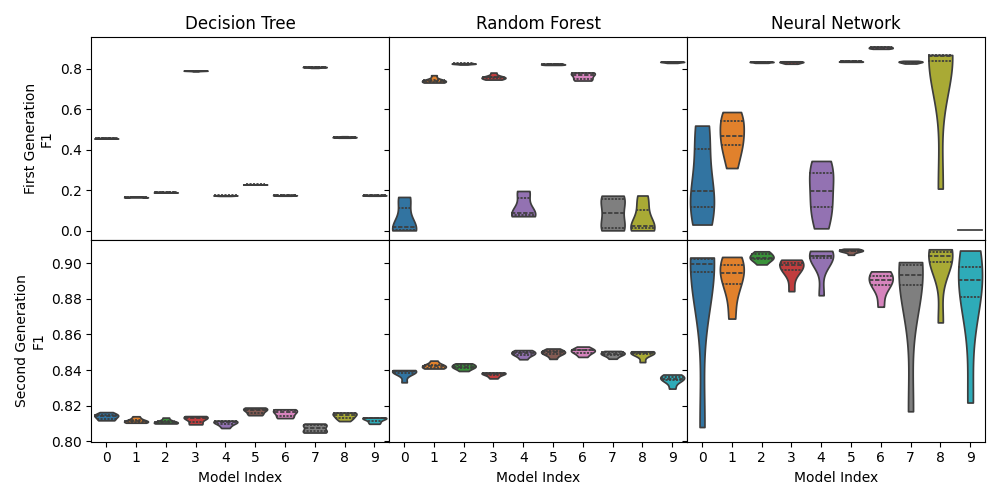
\includegraphics[width=\textwidth]{images/model_selection.png}
    \caption{Accuracy distribution of each model configuration tested during the model selection process.}
    \label{fig:model_selection}
\end{figure}

\begin{figure}[H]
    \centering
    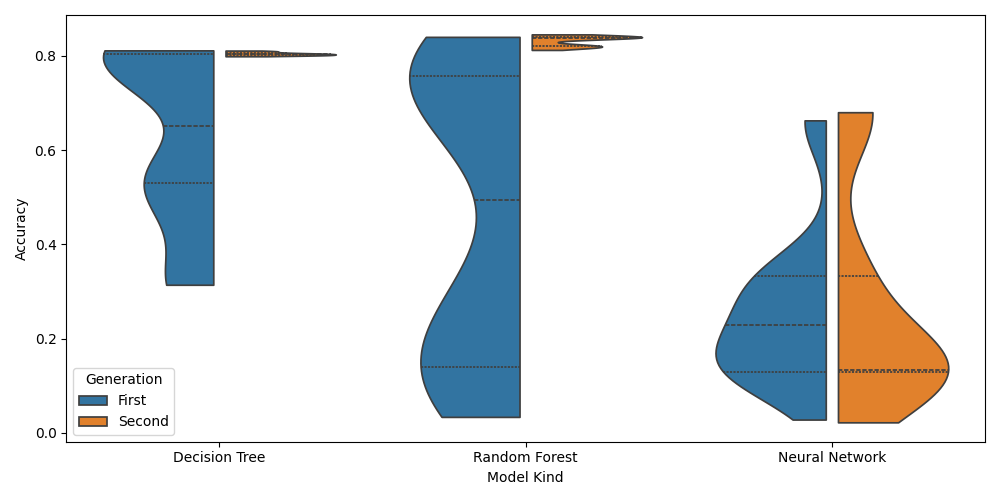
\includegraphics[width=\textwidth]{images/accuracy_distribution.png}
    \caption{Accuracy distribution of each model category.}
    \label{fig:accuracy_distribution}
\end{figure}
\begin{multicols}{2}

Among the models tested in this work, 
the best one was the random forest followed
by the decision tree and then the neural network.
The best models for each kind are shown in
\autoref{tab:best_model_per_kind} and their
respective hyperparameters are shown in
\autoref{tab:hyperparameters_best_decision_tree},
\autoref{tab:hyperparameters_best_random_forest} and
\autoref{tab:hyperparameters_best_neural_network}.

\begin{table}[H]
\centering
\capstart
\begin{tabularx}{0.48\textwidth}{|X|r|}
\hline
Model Name & Mean F1 \\
\hline
\texttt{decision\_tree-G0-9} & 81.08\% \\
\texttt{random\_forest-G0-0} & 83.65\% \\
\hline
\end{tabularx}
\caption{Best models for each kind}
\label{tab:best_model_per_kind}

\end{table}


\begin{table}[H]
\centering
\capstart
\begin{tabularx}{0.48\textwidth}{|X|l|}
\hline
Hyperparameter & Value \\
\hline
\texttt{criterion} & gini \\
\texttt{splitter} & best \\
\texttt{max\_depth} & 1000 \\
\texttt{min\_impurity\_decrease} & 1e-06 \\
\texttt{class\_weight} & balanced \\
\hline
\end{tabularx}
\caption{Hyperparameters used for model \texttt{decision\_tree-G1-5}.}
\label{tab:hyperparameters_best_decision_tree}

\end{table}

\begin{table}[H]
\centering
\capstart
\begin{tabularx}{0.48\textwidth}{|X|l|}
\hline
Hyperparameter & Value \\
\hline
\texttt{n\_estimators} & 100 \\
\texttt{preprocessor} & tfidf \\
\texttt{criterion} & log\_loss \\
\texttt{max\_depth} & 100 \\
\texttt{min\_impurity\_decrease} & 1e-06 \\
\texttt{n\_jobs} & -1 \\
\texttt{class\_weight} & balanced \\
\hline
\end{tabularx}
\caption{Hyperparameters used for model \texttt{random\_forest-G0-0}.}
\label{tab:hyperparameters_best_random_forest}

\end{table}

\begin{table}[H]
\centering
\capstart
\begin{tabularx}{0.48\textwidth}{|X|l|}
\hline
Hyperparameter & Value \\
\hline
\texttt{network} & ff\_tfidf \\
\texttt{base\_size} & 32 \\
\texttt{depth} & 1 \\
\texttt{epochs} & 20 \\
\texttt{patience} & 2 \\
\texttt{dropout} & 0.5 \\
\texttt{batchnorm} & False \\
\texttt{batch\_size} & 32 \\
\texttt{lr} & 0.001 \\
\texttt{optimizer} & adam \\
\hline
\end{tabularx}
\caption{Hyperparameters used for model \texttt{neural\_network-G1-3}.}
\label{tab:hyperparameters_best_neural_network}

\end{table}


The best model was selected based on 
the average accuracy obtained in the
cross-validation. The accuracy distribution
of this model was compared to the other
models with a Wilcoxon signed-rank test,
some models were not significantly different 
($p>0.05$) from the best model and they 
are listed in \autoref{tab:best_models}.

\begin{table}[H]
    \centering
    \begin{tabular}{|l|r|}
        \hline
        \textbf{Model ID} & \textbf{Average Accuracy} \\
        \hline
        \texttt{neural\_network-G1-0} & $82.00\%$ \\
        \hline
    \end{tabular}
    \caption{Best model (first row) and models not significantly different from the best model.}
    \label{tab:best_models}
\end{table}

As we can see in 
\autoref{fig:accuracy_distribution}, the random
forest is the most susceptible to
hyperparameter changes, as it has the widest
accuracy distribution, while the decision tree
is the least susceptible, with the smallest
accuracy distribution.

\begin{table}[H]
\centering
\begin{tabularx}{0.48\textwidth}{|X|r|}
\hline
Metric & Value \\
\hline
Accuracy & 84.59\% \\
Precision & 75.03\% \\
Recall & 79.53\% \\
F1 & 76.66\% \\
\hline
\end{tabularx}
\caption{Metrics relative to the best model \texttt{random\_forest-G1-8} evaluated on the test set.}
\label{tab:best_model_metrics_test}

\end{table}


\begin{figure}[H]
    \centering
    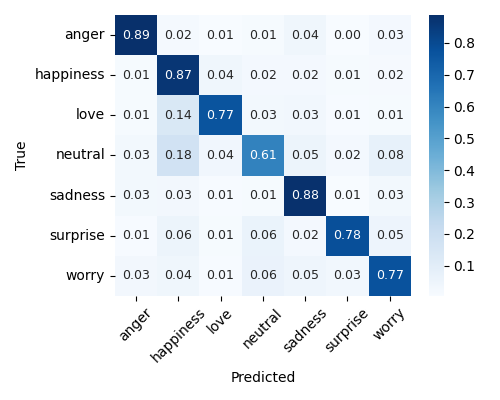
\includegraphics[width=0.48\textwidth]{images/best_model_confusion_matrix_test.png}
    \caption{Confusion matrix of the best model.}
    \label{fig:confusion_matrix_test}
\end{figure}

The best model was also tested on a subset of the
test set, composed of only the instances that
were taken from the CrowdFlower dataset. The
results can be compared to the results obtained
by those of the paper from Batbaatar et al.
\cite{emotion_recognition_from_text}. The metrics
obtained are shown in 
\autoref{tab:best_model_metrics_crowdflower_test}.
We can see that the model has a worse performance
on this subset compared to the model from the
paper (51.1\% of accuracy), this can be 
explained by the much more complex model used
by the authors: a deep LSTM and CNN network with 
different kinds of embedding that extract both 
semantic information and sentiment information 
from the text.

\begin{table}[H]
\centering
\capstart
\begin{tabularx}{0.48\textwidth}{|X|r|}
\hline
Metric & Value \\
\hline
Precision & 37.79\% \\
Recall & 27.43\% \\
F1 & 15.86\% \\
\hline
\end{tabularx}
\caption{Metrics relative to the best model \texttt{neural\_network-G1-5} evaluated on the crowdflower test set.}
\label{tab:best_model_metrics_crowdflower_test}

\end{table}

